\documentclass[13pt]{article}

\usepackage[caption=false,font=footnotesize]{subfig}
\usepackage{graphicx}
\newcommand\figref{Fig.~\ref}

\begin{document}

\section{Notes for My Paper}
In questo capitolo....


\subsection{How to handle topicalization}
 nella mia sottosezione scrivo....
 
\subsection{Mood}

\section{Nuovo Capitolo}
Nuovo capitolo presento una papera \figref{fig:duck}

\begin{figure}[h]
	\centering
	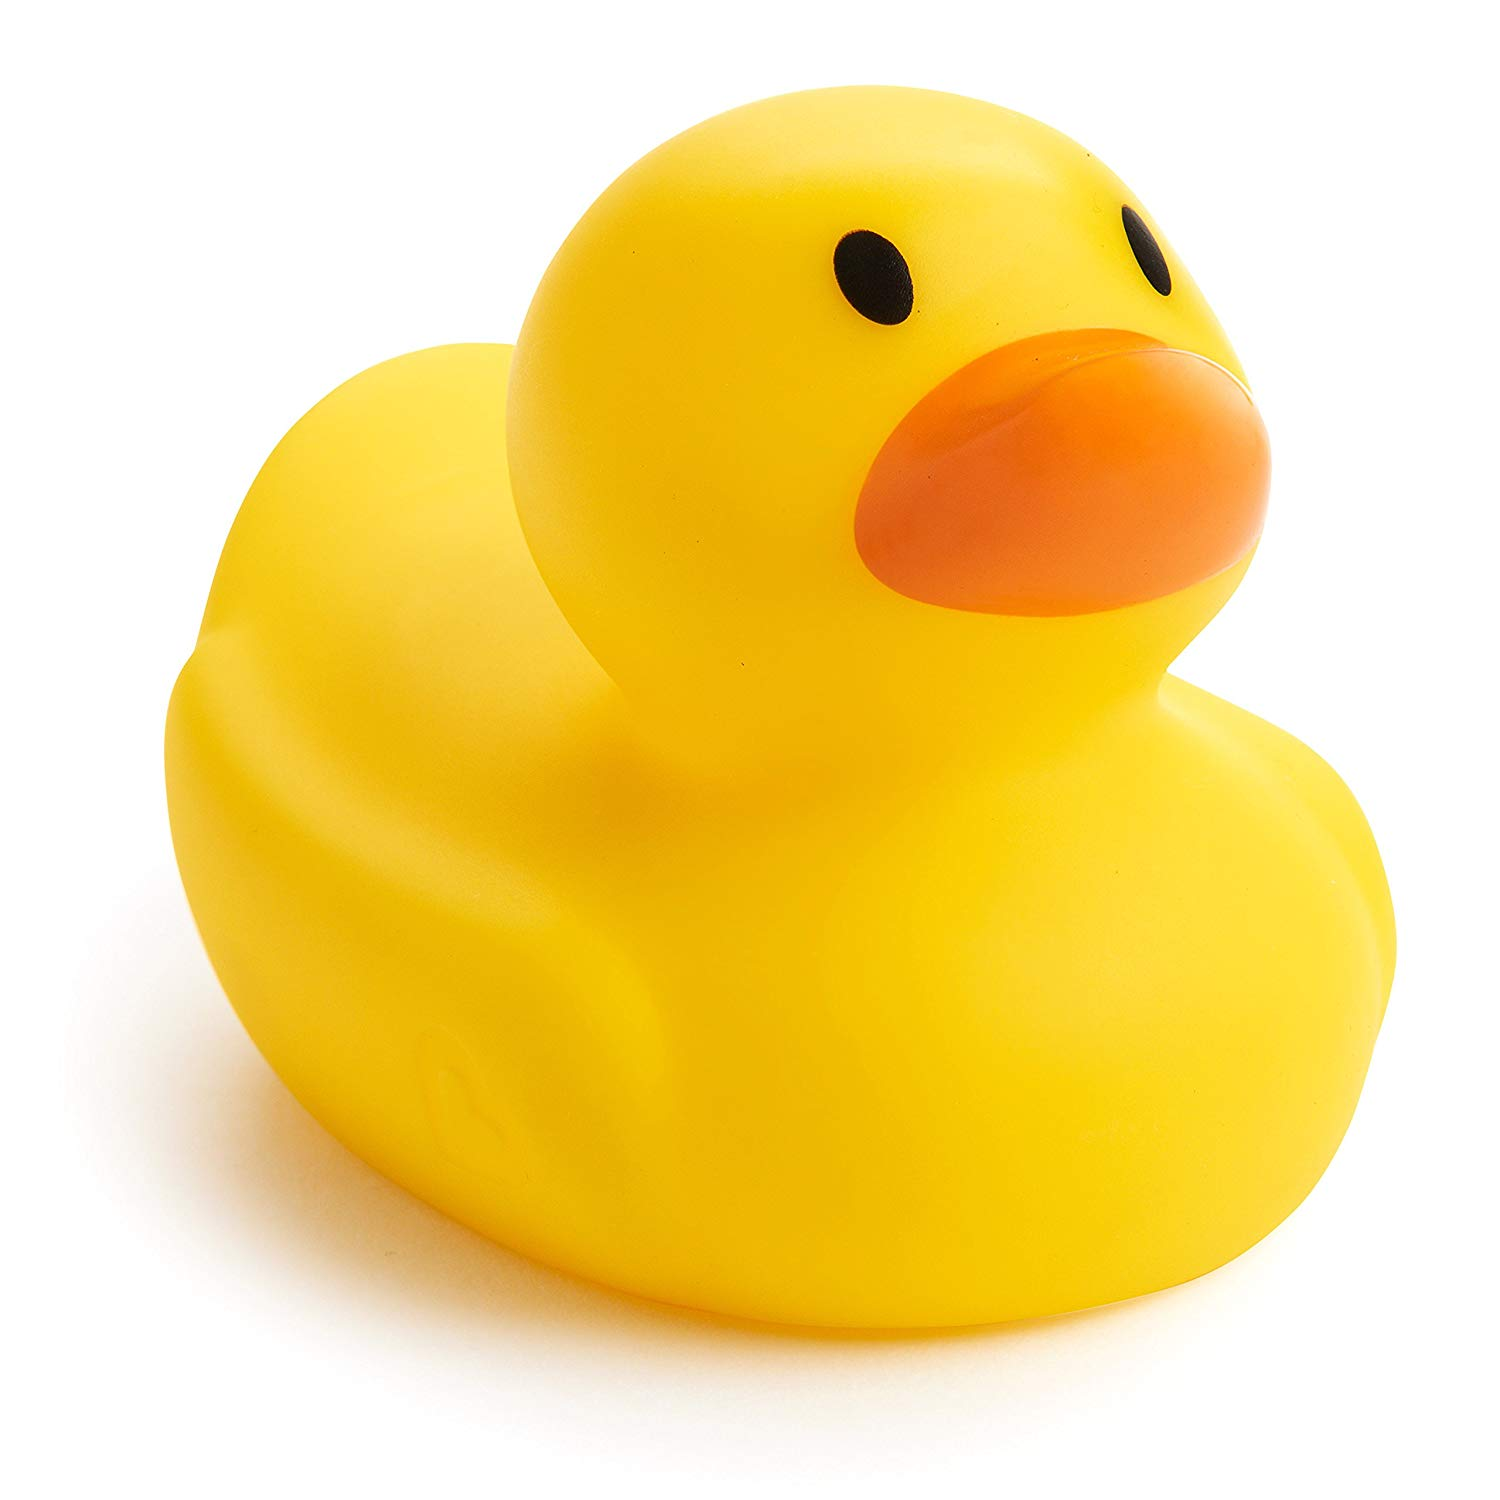
\includegraphics[width=0.9\columnwidth]{Images/duck}
	\caption{La mia papera}
	\label{fig:duck}
\end{figure}

Nella chimica analitica strumentale, tecnica di purificazione e separazione di sostanze, anche molto simili, presenti in miscele liquide o gassose anche complesse, che sfrutta la diversa distribuzione dei componenti fra due fasi, una legata a un supporto ( fase stazionaria ) e l'altra che percorre la prima insieme alla miscela ( fase mobile ): i componenti separati sono determinati qualitativamente e quantitativamente per mezzo di opportuni rivelatori.

\end{document}